\documentclass[12pt]{article}
\usepackage[left=1in,top=1in,right=1in,bottom=1in]{geometry}
\usepackage{graphicx}
\usepackage{titling}
\usepackage[bookmarks=true,colorlinks=true, linkcolor=red, citecolor=cyan]{hyperref}

\setlength{\droptitle}{-1.0in}   % This is your set screw


\begin{document}


\title{FQL++ IDE Manual}
\author{Ryan Wisnesky}
\date{\today}

\maketitle

%\begin{abstract}
%This manueal describe FQL IDE to database practitioners without backgrounds in category theory.
%\end{abstract}
\vspace{-0.5in}

\begin{footnotesize}
\tableofcontents
\end{footnotesize}
\newpage

\section{Introduction}

FQL++, a successor to FQL, the {\it functorial query language}, implements {\it functorial data migration}.  The FQL++ IDE is an open-source java program that provides a code editor for and visual representation of FQL++ programs.  A screen shot of the initial screen of the FQL++ IDE is shown below.  As FQL++ succeeds FQL, readers are recommended to first familiarize themselves with FQL and the FQL IDE.

\begin{center}
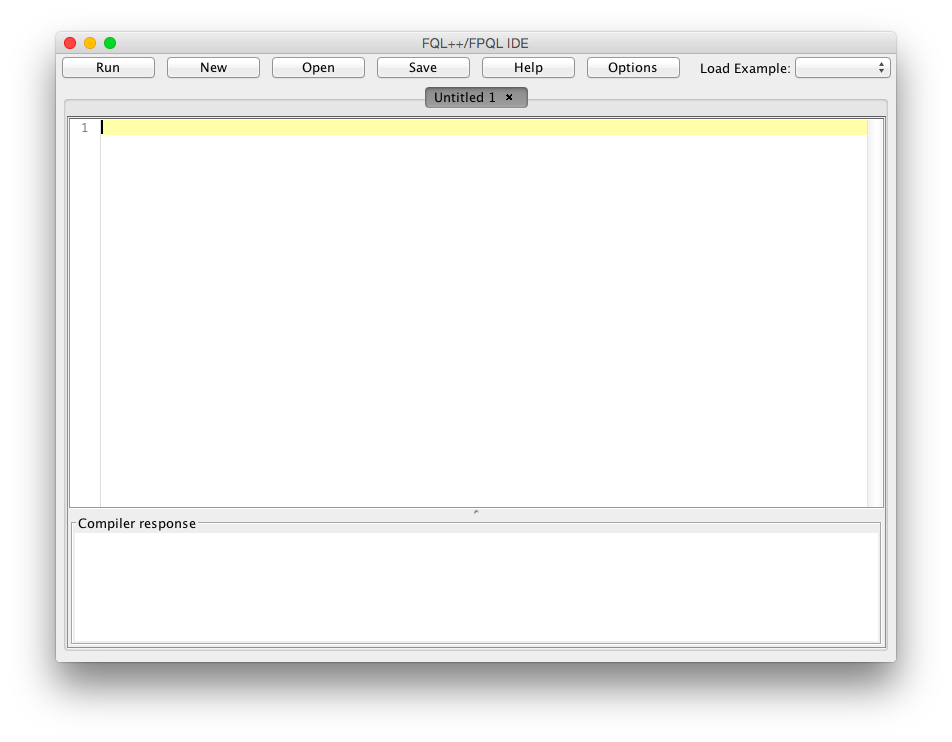
\includegraphics[width=5in]{initial}
\end{center}

The FQL++ IDE is a multi-tabbed text file editor that supports saving, opening, copy-paste, etc.  Associated with each editor is a ``compiler response'' text area that displays an error message if execution fails.  The built-in FQL++ examples can be loaded by selecting them from the ``load example'' combo box in the upper-right.  In the rest of this tutorial we will refer to these examples.  Compilation can be aborted with the ``abort'' button in the Tools menu.  Abort is ``best effort'' and can leave FQL++ in an inconsistent state; it is provided to allow users to terminate FQL++ gracefully.  

To run FQL++ with more than the default 64mb heap, you must use command line options:
\begin{verbatim}
java -Xms512m -Xmx2048m -jar fql_lib.jar
\end{verbatim}

\newpage

\section{FQL++ Basics}

Unlike FQL, which focuses on SQL compatibility and ``attributes'', the focus of FQL++ is on the ``pure'' functorial data model.  That is, the core concepts in FQL++ are {\it categories}, {\it functors}, and {\it natural transformations}, and an FQL++ program is an ordered list of uniquely named {\it declarations} of these three kinds.  Comments in FQL++ are Java style, either ``//'' or ``/* */''. Negative integers must be quoted with double quotes.

\subsection{Categories}

Select the ``employees'' examples.  This action will create a new tab containing the following FQL++ code:
\begin{verbatim}
category S = { 
 objects
 	Employee, Department;
 arrows
	  manager   : Employee -> Employee,
	  worksIn   : Employee -> Department,
	  secretary : Department -> Employee;
 equations  
  	Employee.manager.worksIn = Employee.worksIn,
  	Department.secretary.worksIn = Department,
  	Employee.manager.manager = Employee.manager; 
}\end{verbatim}
This declaration defines a category presentation $S$ consisting of two {\it objects}, three {\it arrows}, and three {\it equations}.  Unlike FQL, in FQL++ {\it there are no attributes.}  In relational terminology, this means that   
\begin{itemize}
\item Each node corresponds to an {\it entity type}.  In this example, the two types of entities are employees and departments.
\item Each arrow $f : X \to Y$ corresponds to a total function $f$ from entities of type $X$ to entities of type $Y$.   In this example, manager maps employees to employees, worksIn maps employees to departments, and secretary maps departments to employees.
\item The equations specify the data integrity constraints that must hold of all instances that conform to this schema.  FQL++ uses equalities of paths as constraints.  A path $p$ is defined inductively as
$$
p ::= node \ | \ p.arrow
$$ 
Intuitively, the meaning of ``.'' is composition.  In this example, the constraints are: 1) every employee must work in the same department as his or her manager; 2) every departmental secretary must work for that department; and 3) there are employees and managers, but not managers of managers, managers of managers of managers, etc.
\end{itemize}
The FQL++ IDE can render categories into a graphical form.  Press ``run'', and select the category $S$ from the viewer:

\begin{center}
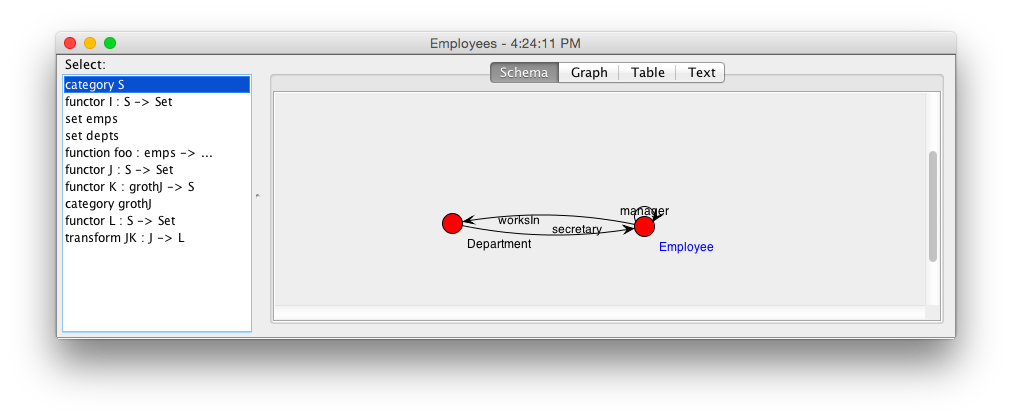
\includegraphics[width=6in]{schema}
\end{center}

Note that the three sections, ``objects'', ``arrows'', and ``equations'' are ended with semi-colons, and must appear in that order, even when a section is empty.  The ``text'' tab prints the category that the presentation denotes.

\subsubsection{Infinite Categories}

FQL++ requires all category presentations to denote finite categories.  Such category presentations can be cyclic, provided they have ``finitizing'' equations, such as above.  

\subsection{Functors}
Next, load the ``delta'' example.  It defines two categories, $C$ and $D$, and a functor $F$ from $C$ to $D$:

 \begin{minipage}{0.4\textwidth}
\begin{verbatim} 


 category C = {
 objects 
	T1, T2, string, int;
 arrows
	t1_ssn    : T1 -> string,
	t1_first  : T1 -> string,
	t1_last   : T1 -> string,
	t2_first  : T2 -> string,
	t2_last   : T2 -> string,
	t2_salary : T2 -> int;
 equations; 
}    \end{verbatim}
  \end{minipage}
%  \quad
   \hspace{.5in} $\to_F$ \hspace{.5in}
  \begin{minipage}{0.4\textwidth}
\begin{verbatim} 

category D = {
 objects 
	T, string, int;
 arrows
	ssn0    : T -> string,
	first0  : T -> string,
	last0   : T -> string,
	salary0 : T -> int;
 equations;
}   
\end{verbatim} \end{minipage}
  
\begin{verbatim}



functor F = {
 objects 
	T1 -> T,
	T2 -> T,
	string -> string,
	int -> int;
 arrows
	t1_ssn    -> T.ssn0,
	t1_first  -> T.first0,
	t2_first  -> T.first0,
	t1_last   -> T.last0,
	t2_last   -> T.last0,
	t2_salary -> T.salary0;
} : C -> D
\end{verbatim}
A functor $F : C \to D$ between finitely presented $C$ and $D$ consists of two parts:
\begin{itemize}
\item a mapping from the objects in $C$ to the objects in $D$
\item a mapping from the arrows in $C$ to paths in $D$
\end{itemize}
A functor must respect the equations of $C$ and $D$: if $p_1$ and $p_2$ are equal paths in $C$, then $F(p_1)$ and $F(p_2)$ must be equal paths in $D$.  If this condition is not met, FQL++ will throw an exception.  Our example mapping is rendered in the viewer as follows:

\begin{center}
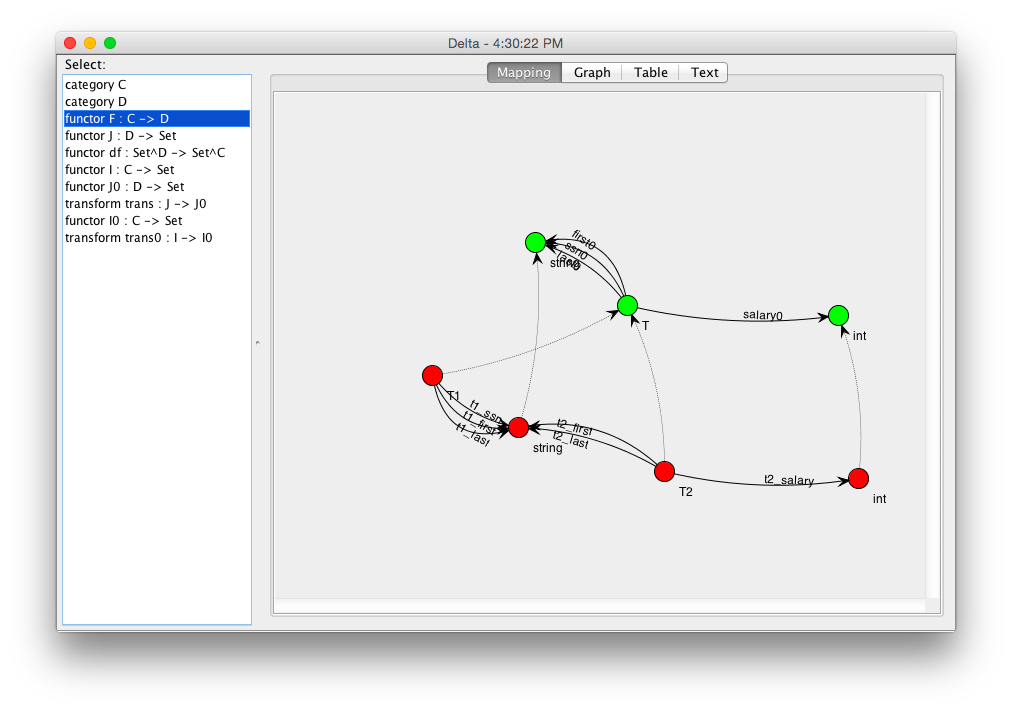
\includegraphics[width=4in]{mapping}
\end{center}

An identity mapping can be formed using the keyword ``id'' as follows:
\begin{verbatim}
functor F = id C
\end{verbatim}
Mappings can be composed using the keyword ``;'' (parenthesis required) as follows:
\begin{verbatim}
functor F = (G ; H)
\end{verbatim}

\subsubsection{Instances}

Continuing with the built-in ``employees'' example, we see that it also contains FQL++ code that defines an instance -- a set-valued functor -- of the category $S$ defined previously:

\begin{verbatim}
functor I = {
 objects
	  Employee -> { 101, 102, 103 },
	  Department -> { q10, x02 };
 arrows
	  manager -> { (101, 103), (102, 102), (103, 103) } : {101,102,103} -> {101,102,103},
	  worksIn -> { (101, q10), (102, x02), (103, q10) } : {101,102,103} -> {q10,x02},
	  secretary -> { (q10, 101), (x02, 102) } : {q10,x02} -> {101,102} ;
} : S -> Set
\end{verbatim}

This declaration defines an instance $I$ that conforms to category $S$.  This means that
\begin{itemize}
\item To each node/entity type corresponds a set of IDs.  In this example, the employee IDs are 101, 102, and 103, and the departmental IDs are q10 and x02.
\item Each arrow $f : X \to Y$ corresponds to a function that maps IDs of entity type $X$ to IDs of entity type $Y$.  
\end{itemize}

To visualize this instance, press ``run'', select the instance from the viewer list, and click the ``joined'' tab:

\begin{center}
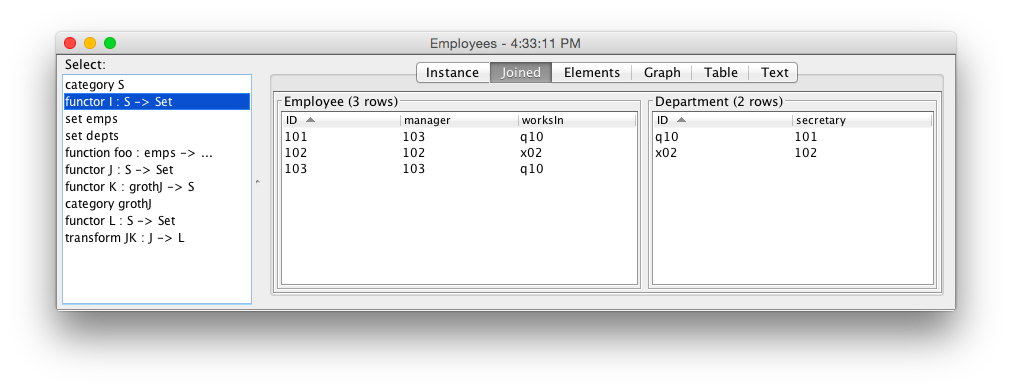
\includegraphics[width=5.5in]{instance}
\end{center}

To enter a string that contains spaces, simply quote it.  

\subsubsection{Category of Elements}

Provided the ``Elements'' option is enabled, the ``Elements'' tab in an instance displays the instance as a category, ``the category of its elements''.  In this view, nodes are entities and arrows are foreign-key correspondences. 

\subsubsection{Natural Transformations (database homomorphisms)}

For each category presentation $T$ and $T$-instances $I$,$J$, a {\it (natural) transformation} $f : I \Rightarrow J$ is a database homomorphism from $I$ to $J$: for each node $n \in T$, $f_n$ is a constraint respecting function from $I_n$ IDs to $J_n$ IDs.  Transformations are illustrated in the ``Delta'' example.  
\begin{verbatim}
functor J = {
 objects 
	  T -> { XF667, XF891, XF221 },
	  string -> { "115-234", "112-988", "198-887", Bob, Sue, Alice, Smith, Jones },
	  int -> { 250, 100, 300 };
 arrows
	  ssn0    -> { (XF667, "115-234"),(XF891,"112-988"),(XF221,"198-887") },
	  first0  -> { (XF667,Bob),(XF891,Sue),(XF221,Alice) },
	  last0   -> { (XF667,Smith),(XF891,Smith),(XF221,Jones) },
	  salary0 -> { (XF667,250),(XF891,300),(XF221,100) };
} : D -> Set

functor J0 = {
 objects 
	  T -> { XF66,XF89,XF22, xxx },
	  string -> { "115-23", "112-98", "198-88", Bo, Su, Alic, Smit, Jone, xxx },
	  int -> { 25, 10, 30, 0 };
 arrows
	  ssn0    -> { (XF66, "115-23"),(XF89,"112-98"),(XF22,"198-88"), (xxx,"xxx") },
	  first0  -> { (XF66,Bo),(XF89,Su),(XF22,Alic),(xxx, "xxx" )},
	  last0   -> { (XF66,Smit),(XF89,Smit),(XF22,Jone), (xxx, "xxx") },
	  salary0 -> { (XF66,25),(XF89,30),(XF22,10), (xxx, 0) };
} : D -> Set

transform trans = {
 objects 
 	T -> {(XF667,XF66),(XF891,XF89),(XF221,XF22)},
 	string -> { ("115-234","115-23"), ("112-988","112-98"), ("198-887","198-88"), 
 	            (Bob,Bo), (Sue,Su), (Alice,Alic), (Smith,Smit), (Jones,Jone) },
 	int -> {(250,25),(100,10),(300,30)};
} : (J: D -> Set) -> (J0: D -> Set)  
\end{verbatim}
Note that the types of $J$ and $J_0$ are required when defining $trans$ above, and that $\to$ is used in FQL++ code rather than $\Rightarrow$.

\newpage
\subsection{Data Migration}

Associated with a functor between finitely presented categories $F : C \to D$ are three data migration operators:
\begin{itemize}
\item $\Delta_F$, taking $D$ instances to $C$ instances, roughly corresponding to projection
\item $\Pi_F$, taking $C$ instances to $D$ instances, roughly corresponding to join
\item $\Sigma_F$, taking $C$ instances to $D$ instances, roughly corresponding to union
\end{itemize}


\subsubsection{Delta}

Continuing with the ``delta'' example, we see that the FQL++ program also defines a $D$-instance $J$, and computes $I := \Delta_F(J)$.  In effect, we have projected the columns salary0 and last0 from $J$.  

\begin{verbatim}
functor df = delta F

functor I = apply df on object J
\end{verbatim}

Graphically, we have

\begin{center}
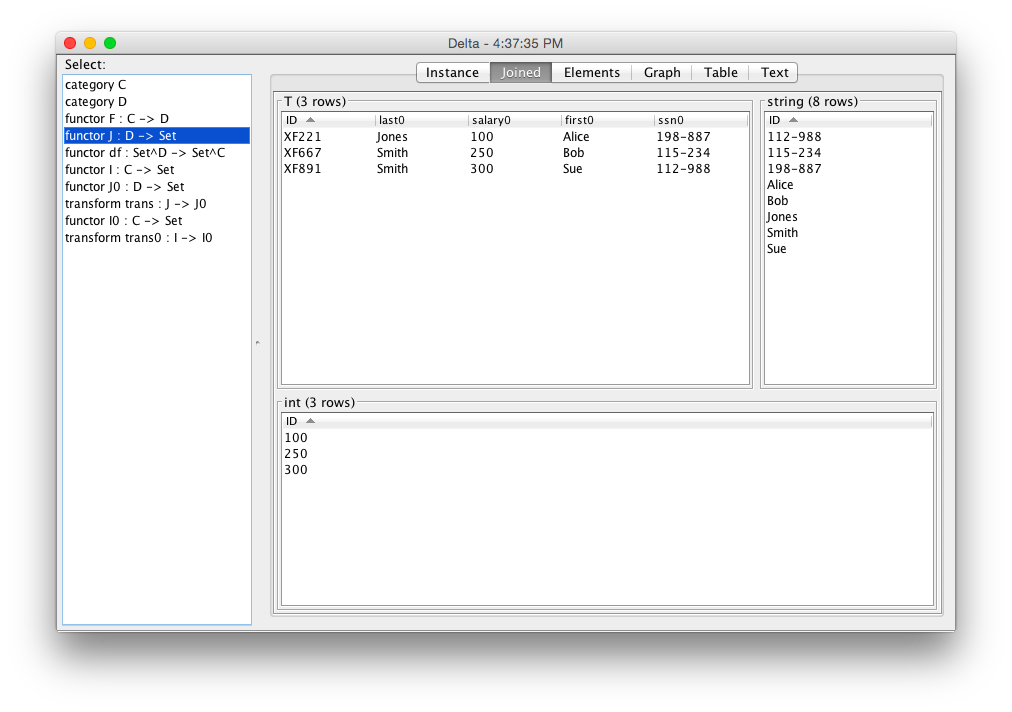
\includegraphics[width=6in]{deltaJ}

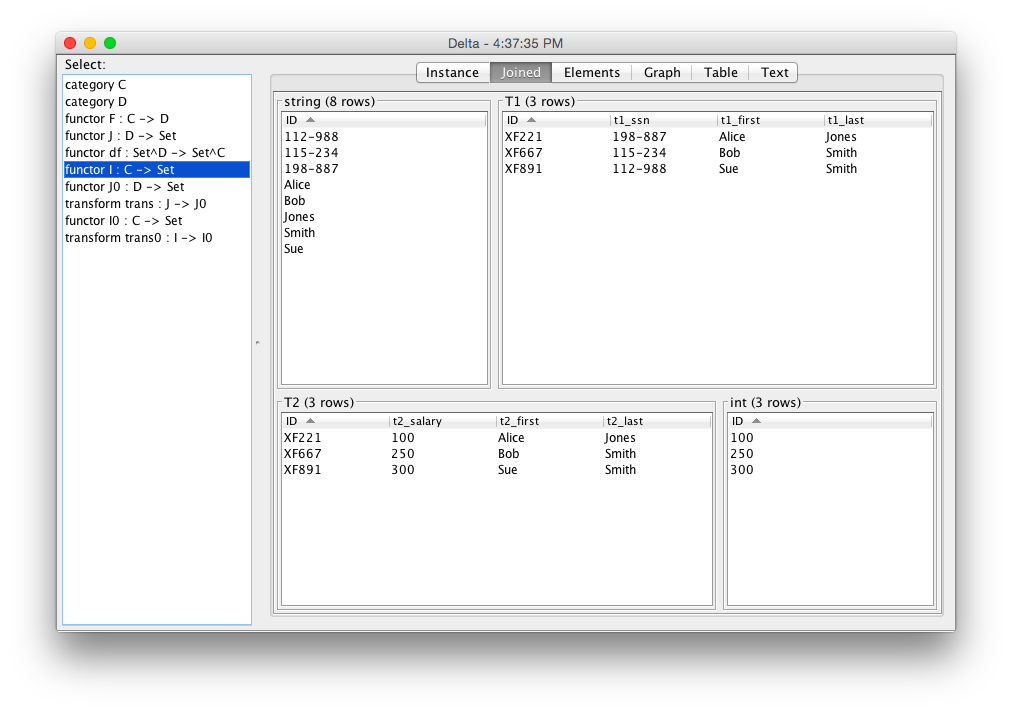
\includegraphics[width=6in]{deltaI}
\end{center}


\subsubsection{Pi}

Load the ``pi'' example:

 \begin{minipage}{0.4\textwidth}
\begin{verbatim} 


 category C = {
 objects 
 	c1, 
 	c2,
 	string;
 arrows
	att1 : c1 -> string,
	att2 : c1 -> string, 
	att3 : c2 -> string;
 equations;
}
    \end{verbatim}
  \end{minipage}
%  \quad
   \hspace{.5in} $\to_F$ \hspace{.5in}
  \begin{minipage}{0.4\textwidth}
\begin{verbatim} 

category D = {
 objects 
 	d,
 	string;
 arrows
 	a1 : d -> string, 
 	a2 : d -> string, 
 	a3 : d -> string;
 equations;
}

\end{verbatim} \end{minipage}
\begin{verbatim}
functor F = {
 objects 
 	c1 -> d, c2 -> d, string -> string;
 arrows
	  att1 -> d.a1,  att2 -> d.a2, att3 -> d.a3;
} : C -> D

\end{verbatim}
This example defines an instance $I : C$ and computes $J := \Pi_F(I)$:
\begin{verbatim}
functor J = apply pi F on object I
\end{verbatim}
Graphically, this is rendered as:

\begin{center}
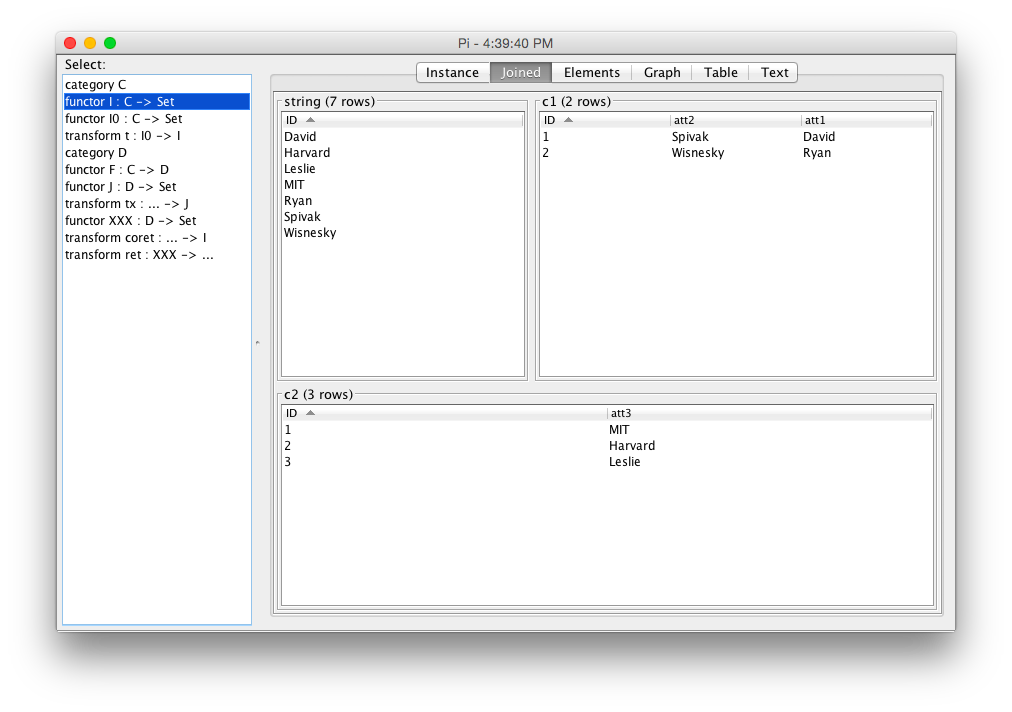
\includegraphics[width=5in]{piI}

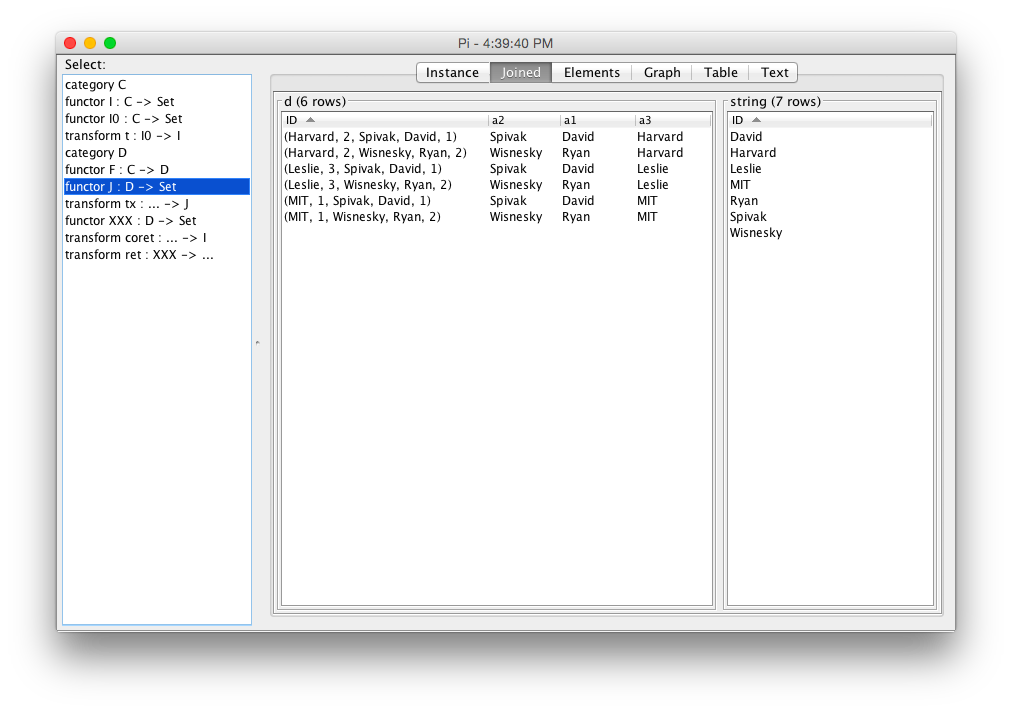
\includegraphics[width=5in]{piJ}
\end{center}

We see that we have computed a cartesian product.  Note that unlike FQL, the IDs created by FQL++ have structure.  The exact way to create new IDs is set by a menu option: fresh, corresponding to new IDs, summary, shown above, and lineage, which is the most verbose.

\subsubsection{Sigma}


Load the ``sigma'' example:

 \begin{minipage}{0.4\textwidth}
\begin{verbatim} 


category C = {
	objects 
		Amphibian,
		LandAnimal,
		WaterAnimal,
		string;
	arrows
		attA : Amphibian -> string, 
		attL:LandAnimal-> string, 
		attW:WaterAnimal->string,
		IsAL:Amphibian->LandAnimal,
		IsAW:Amphibian->WaterAnimal;
	equations;
} \end{verbatim}
  \end{minipage}
%  \quad
   \hspace{.5in} $\to_F$ \hspace{.5in}
  \begin{minipage}{0.4\textwidth}
\begin{verbatim} 
category D ={
	objects 
		yAmphibian,
		yLandAnimal,
		yWaterAnimal,
		yAnimal,
		ystring;
	arrows
		yattA:yAmphibian -> ystring, 
		yattL:yLandAnimal-> ystring, 
		yattW:yWaterAnimal->ystring,
		yIsAL:yAmphibian->yLandAnimal,
		yIsAW:yAmphibian->yWaterAnimal,
		yIsALL:yLandAnimal->yAnimal,
		yIsAWW:yWaterAnimal->yAnimal;
	equations
		yAmphibian.yIsAL.yIsALL=
		yAmphibian.yIsAW.yIsAWW;
}
\end{verbatim} \end{minipage}
\begin{verbatim}
functor F = {
	objects 
		Amphibian->yAmphibian,
		LandAnimal->yLandAnimal,
		WaterAnimal->yWaterAnimal,
		string->ystring;
	arrows
		attA -> yAmphibian.yattA, 
		attL -> yLandAnimal.yattL, 
		attW -> yWaterAnimal.yattW,
		IsAL -> yAmphibian.yIsAL,
		IsAW -> yAmphibian.yIsAW;
} : C -> D
\end{verbatim}
This example defines an instance $I : C$ and computes $\Sigma_F(I)$:
\begin{verbatim}
functor sigma_FI = apply sigma F on object I
\end{verbatim}
Graphically, this is rendered as:

\begin{center}
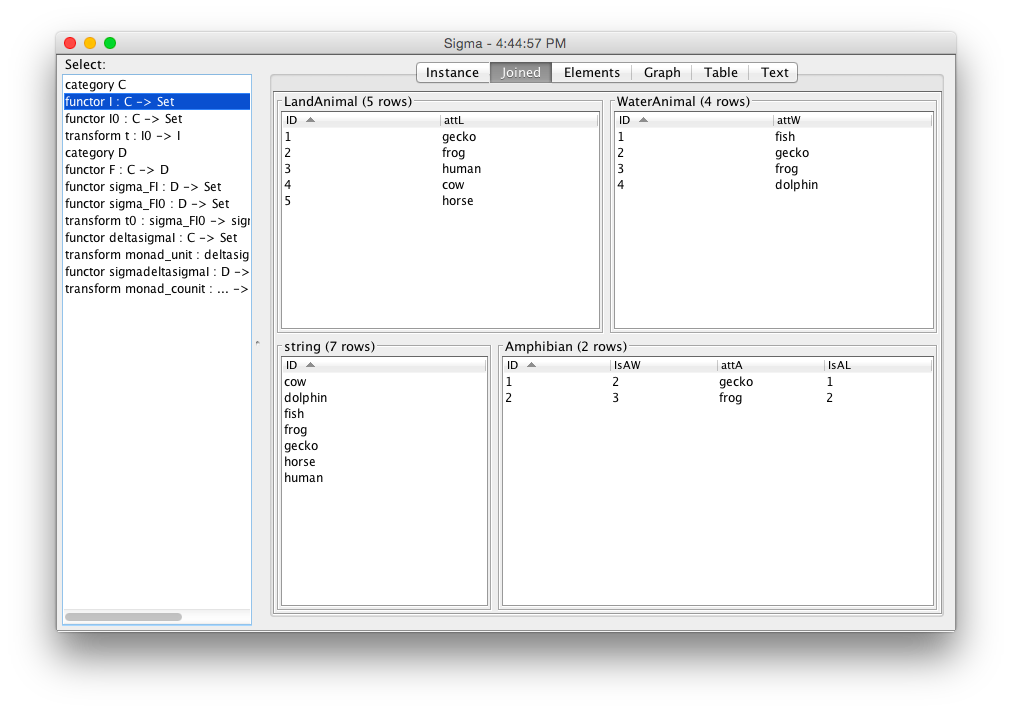
\includegraphics[width=5in]{sigmaI}
\vspace{-.2in}
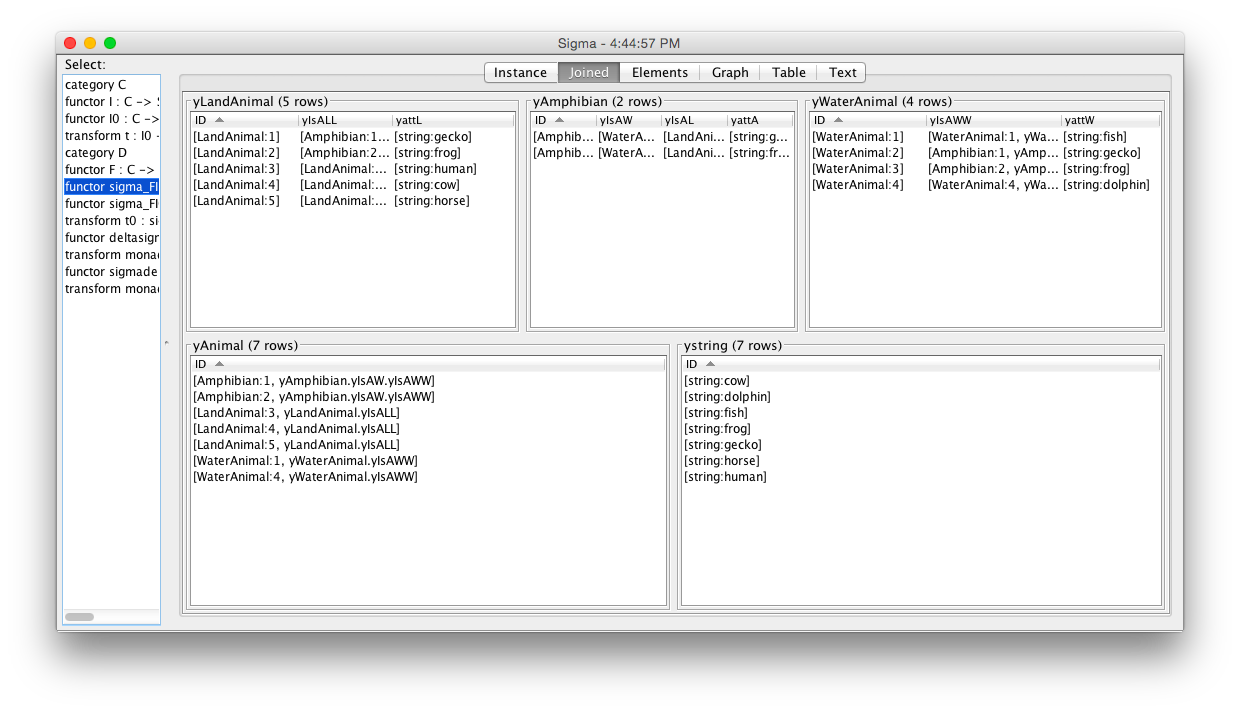
\includegraphics[width=5in]{sigmaJ}
\end{center}
\vspace{-.2in}
As with Pi, there are three ways for FQL++ to create fresh IDs in the target instance, and these are configured in the options menu.

\subsubsection{Data Migration on Transformations}

If $f : I \Rightarrow J$ is a transformation, then so is $\Delta_F(f) : \Delta_F(J) \Rightarrow \Delta_F(I)$, $\Sigma_F(f) : \Sigma_F(I) \Rightarrow \Sigma_F(J)$, $\Pi_F(f) : \Pi_F(f) : \Pi_F(I) \Rightarrow \Pi_F(J)$.  See the All Syntax example for details.

\subsubsection{Units and Co-units}

For every $F$ and $I$, there are canonical transforms $return : I \Rightarrow \Delta_F(\Sigma_F(I))$ and $coreturn : \Sigma_F(\Delta_F(I)) \Rightarrow I$, as well as canonical transforms $return : I \Rightarrow \Pi_F(\Delta_F(I))$ and $coreturn : \Delta_F(\Pi_F(I)) \Rightarrow I$.  These transforms come from the mathematical theory of {\it monads}.  They are illustrated in the Sigma and Pi examples.

\subsection{Categorical Combinators}

FQL++ contains programming capabilities in the guise of {\it categorical combinators}.  Intuitively, these combinators are a standard functional programming language similar to e.g., point-free Haskell. Their semantics derives from the fact that the category of categories  is bi-cartesian closed, and for each $T$, the category of $T$-instances is a topos.  As these combinators are similar to the combinators in FQL, we do not repeat definitions here; instead, we just list all possible syntax.  See the FQL IDE manual for descriptions of products, co-products, exponentials, and sub-object classifiers.

\subsubsection{Programming with Categories and Functors}

\begin{verbatim}

category c1 = void
category c2 = unit
category c3 = (c2 + c2)
category c4 = (c2 * c2)
category c5 = (unit ^ void)
category c6 = Set
category C  = {objects; arrows; equations;}

functor f1 = id unit
functor f2 = (f1 ; f1)
functor f4 = iso1 c4 c5
functor f6 = iso2 c4 c5
functor f7 = (fst c3 c3 * snd c3 c3) 
functor f8  = (inl c3 c3 + inr c3 c3) 
functor f9  = curry eval c3 c3 
functor f10 = {objects; arrows;} : C -> C //mapping
functor f20 = {objects; arrows;} : C -> Set //instance
functor f13 = (f20 ^ f20) 
functor f14 = delta f10
functor f15 = sigma f10
functor f16 = pi f10
functor f17 = apply f14 on object f20
functor f18 = prop C
functor t21 = void C Set //need Set here
functor t22 = unit C Set //need Set here
functor f3 = ff unit
functor f5 = tt unit

category c6x = dom f1
category c7x = cod f2
\end{verbatim}


\subsubsection{Programming with Functors and Transformations}

\begin{verbatim}

transform t0 = {objects;} : (f20:C->Set) -> (f20:C->Set) 
//must have dom and cod of functors above 
transform t1 = id f20
transform t2 = (t1 ; t1) 
transform t3x= (inl f20 f20 + inr f20 f20) 
transform t4x= (fst f20 f20 * snd f20 f20) 
transform t5 = curry eval f20 f20
transform t5x = tt f20
transform t5y = ff f20
transform t6 = apply f14 on arrow t1
transform t7 = true C
transform t8 = false C
transform t9 = and C
transform t7y= or C
transform t7x= not C
transform t8z= implies C
transform t8x= return sigma delta f10
transform t9x= coreturn sigma delta f10
transform t10= return delta pi f10
transform t11= coreturn delta pi f10
transform t12= iso1 f20 f20
transform t13= iso2 f20 f20

functor f19x = dom t1
functor t20x = cod t1
\end{verbatim}
 \newpage
 \section{FQL++ features beyond FQL}
 
The fragment of FQL++ described above is a subset of FQL: the subset containing no attributes.  In exchange for removing attributes, FQL++ contains a number of features that go beyond FQL.

\subsection{Programming with Sets}
FQL++ contains a full programming language for finite sets based on the internal language of a BCCC.  See the 'Sets' example.  These sets and functions can be used anywhere that FQL++ expects a set or function, for example, in an instance declaration.
\begin{verbatim}
/*
 * In FQL++, a *value* is either:
 *
 *  - a string, that must be quoted if it contains spaces or special symbols, like "-".
 *        Numbers are treated as strings in FQL++.
 *  - a unit, written ().
 *  - a boolean, written true or false.
 *  - a pair of two values v1 and v2, written (v1, v2).
 *  - a left or right injection of a value v, written inl v or inr v.
 *  - a (possibly empty) set of values, written {v1, ..., vn}.
 *  - a function, written as a set of pairs with explicit domain and co-domain:
 *        {(x1,y1), ..., (xN,yN)} : {x1, ..., xN} -> {y1, ..., yN}.
 */

//A *set literal* is a set of values, for example: 
set s1 = {foo, bar, "b a z", 7, true, false}
set s2 = {(), inl (), inr (), inl inr 7, (hello,world), {a,b,{c,d},{}}}
set s3 = { {(1,1),(2,4),(3,9)} : {1,2,3} -> {1,4,9}, {(1,1),(2,4),(3,9)} 
  : {1,2,3} -> {1,4,9,10,11,12} }

//A *set* is either a set literal, as above, or a set constructed from
//set literals and +,*,^,void,unit,prop, for example:
set s4 = void // = {}
set s5 = unit // = { () }
set s6 = prop // = { true, false }
set s7 = (unit + unit) // = { inl (), inr () }
set s8 = (prop * prop) // = { (true,true),(true,false),(false,true),(false,false) }
set s9 = (prop ^ unit) // = { ((), true) : {()} -> {true,false}, ((), false) 
  : {()} -> {true,false} }

//a *function literal* is a function value, for example
function f1 = { (1,2),(2,3) } : {1,2} -> {2,3}

//functions can refer to named sets, so we could write instead
set sf = {1,2}
function f2 = { (1,2),(2,3) } : sf -> {2,3}

//a *function* is either a function literal, as above, or a function constructed from
//function literals and tt,ff,fst,snd,(+),(*),(;),eval,curry,char,kernel,iso1,iso2,id
//for example
function f3 = fst {a,b} {c,d} // (a,c) -> a  (a,d) -> a  (b,c) -> b  (b,d) -> d
function f4 = inl {a,b} {c,d} // a -> inl a, b -> inl b
function f5 = id {a,b} // a -> a, b -> b
function f6 = (f5 ; f5) // = f5
function pair_eta = (fst {a,b} {c,d} * snd {a,b} {c,d}) // = id
function sum_eta = (inl {a,b} {c,d} + inr {a,b} {c,d}) // = id
function exp_eta = curry eval {a} {b} // = id
function f7 = char {(1,a),(2,b)} : {1,2} -> {a,b,c} // = a -> true, b -> true
function f8 = kernel f7 // = {(a, a),  (b, b)} : {a, b} -> {a, b, c}
function f9 = iso1 {a,b} {1,2} // = a -> 1, b -> 2
function f10 = tt {a}
function f11 = ff {a}
function f12 = true
function f13 = false
function f14 = and
function f15 = or
function f16 = not
function f17 = implies

//Domains, co-domains, and range require that you must name the function, i.e., as f7
set x = dom f7 // = {a,b}
set y = cod f7 // = {true,false}
set z = range f8 // = {a,b}

//the number n denotes the set {0, ..., n-1}
set two = 2
set three = 3
set five = 5
set two_plus_three = (2+3)
function two_plus_three_equals_five = iso1 two_plus_three five
\end{verbatim}

\subsection{The categories $Cat$, $Set$, and $C$-Inst}

In addition to finitely presented categories, FQL++ contains keywords for the category of sets, $Set$, the category of categories, $Cat$, and for each finitely presented $C$, the category $Set^C$.  It is possible to create functors from finitely presented categories to these categories, and, moreover, to create transforms between such functors.  See the ``categories'' example.
\begin{verbatim}
//////////////////
//cat-valued functors
//let C and D be finitely presented categories, and F a mapping
category X = {
 objects 
	c, d;
 arrows
	f : c -> d;
 equations; 
}

functor Y = {
 objects
     c -> C,
     d -> D;
 arrows
	f -> F;
} : X -> Cat

/////////////////////////////////////////////
//Transforms between functors to Set

functor X1 = {
 objects
  c -> {1,2},
  d -> {3,4};
 arrows
  f -> {(1,3),(2,4)};
} : X -> Set

functor X2 = {
 objects
  c -> {a,b,c},
  d -> {d,e,f};
 arrows
  f -> {(a,d),(b,e),(c,f)};
} : X -> Set

transform X1X2 = {
 objects
  c -> {(1,a),(2,b)},
  d -> {(3,d),(4,e)};
} : (X1 : X -> Set) -> (X2 : X -> Set)


/////////////////////////////////////////////
//Transforms between functors to Cat

functor Z = {
 objects
     c -> C,
     d -> C;
 arrows
	f -> id C;
} : X -> Cat

transform ZY = {
 objects
  c -> id C,
  d -> F;
} : (Z : X -> Cat) -> (Y : X -> Cat)


///////////////////////////////////////////////////////////////////////
//Transforms between functors between finitely presented categories

transform FF = {
 objects
  T1 -> T,
  T2 -> T,
  string -> string,
  int -> int;	
} : (F : C -> D) -> (F : C -> D)
\end{verbatim}

A particularly useful application of $Cat$-valued functors is the ability to check commutative diagrams in Cat; see the 'Integration' example.

\subsection{Functors $Set \to Set$, and Monads}
FQL++ has the ability to define functors $Set \to Set$.  Given a monad (on $Set$, or on a finitely presented category), FQL++ can create the associated Kleisli and co-Kleisli categories.  See the 'Monads' example.

\begin{verbatim}
//functors Set -> Set
functor Maybe = { 
 objects
  X -> (unit + X);
 arrows
  f : A -> B -> (inl unit B + (f ; inr unit B));
} : Set -> Set

set Maybe3 = apply Maybe on object 3
set Maybe4 = apply Maybe on object 4

function MaybeF = apply Maybe on arrow {(0,1),(1,2),(2,0),(3,0)} : 4 -> 3

functor Double = {
		objects X->(X*X);
		arrows f:A->B -> ((fst A A; f)*(snd A A; f));
} : Set -> Set

set dbl=apply Double on object {1,2,3}

function f = apply Double on arrow id {1,2,3}

transform ret = {
 objects
  X -> inr unit X;
} : (id Set : Set -> Set) -> (Maybe : Set -> Set)

transform join = {
 objects
  X -> (inl unit X + id (unit + X));
} : ((Maybe ; Maybe) : Set -> Set) -> (Maybe : Set -> Set)

function ret1 = apply ret {1,2,3}
set set1 = apply Maybe on object {1,2,3}
set set2 = apply Maybe on object set1
function joined = apply join set2

category K = kleisli Maybe ret join

////////

category C = {
	objects a,b,c;
	arrows f:a->b,g:b->c;
	equations;
}

functor M = {
	objects a->a, b->c,c->c;
	arrows f->a.f.g,g->c;
} : C -> C

transform eta = {
	objects a->a, b->b.g, c->c;
} : (id C:C->C) -> (M: C->C)

transform mu = {
	objects a->a, b->c, c->c;
} : ((M;M):C->C) -> (M: C->C) 

category M_kleisli = kleisli M eta mu

///////////

category D = {
	objects a,b,c;
	arrows f:a->b,g:b->c;
	equations;
}

functor T = {
	objects a->a, b->a,c->c;
	arrows f->a,g->a.f.g;
} : D -> D

transform epsilon = {
	objects a->a, b->a.f, c->c;
} : (T: D->D) -> (id D:D->D)

transform Delta = {
	objects a->a, b->a, c->c;
} : (T:D->D) -> ((T;T): D->D) 

category CK = cokleisli T epsilon Delta
\end{verbatim}

\subsection{Extended Currying}
 
 FQL++ can convert  a functor $A \times B \to Set$ to a functor $A \to Set^B$ using the keyword CURRY.  See the integration example.
 
 \subsection{Pivot and Un-pivot}
 
 FQL++ can convert a set-valued functor into a category and vice-versa.  See the Employees example.
 


\end{document}